\documentclass[12pt]{report}
\usepackage[margin=1in]{geometry}
\usepackage[english]{babel} 
\usepackage{amsmath,amsfonts,amsthm}
\usepackage{fancyhdr}
\usepackage{enumitem}
\usepackage{indentfirst}
   \usepackage{graphicx}
   \usepackage{float}
      \usepackage{hyperref}
      \usepackage{caption}

\pagestyle{fancy}
\fancyhf{}
\rhead{Eli Schmitter}
\lhead{HW10}
\rfoot{\thepage}

\begin{document}
\section*{5.2}
   \subsection*{2}
   \begin{enumerate}[label={\bf \alph*}]
   \item
      \begin{align*}
         X=73&,n=100\\
         \alpha&=.05\Rightarrow Z_{\alpha/2}=1.96\\
         \widetilde{n}&=100+4=104\\
         \widetilde{p}&=\frac{X+2}{\widetilde{n}}=\frac{75}{104}\\
         \widetilde{p}\pm Z_{\alpha/2}\sqrt{\frac{\widetilde{p}(1-\widetilde{p})}{\widetilde{n}}}&=.7212\pm.08619\\
      \end{align*}
    \item
      \begin{align*}
         X=73&,n=100\\
         \alpha&=.01\Rightarrow Z_{\alpha/2}=2.58\\
         \widetilde{n}&=100+4=104\\
         \widetilde{p}&=\frac{X+2}{\widetilde{n}}=\frac{75}{104}\\
         \widetilde{p}\pm Z_{\alpha/2}\sqrt{\frac{\widetilde{p}(1-\widetilde{p})}{\widetilde{n}}}&=.7212\pm.113\\
      \end{align*}
   \item
      \begin{align*}
      .05&=Z_{\alpha/2}\sqrt{\frac{\widetilde{p}(1-\widetilde{p})}{\widetilde{n}}}\\&\Rightarrow\\
      n&=\frac{\widetilde{p}(1-\widetilde{p})}{\frac{.05}{Z_{\alpha/2}}^2}-4\\
       &=\frac{.7212(1-.7212)}{\frac{.05}{1.96}^2}-4\\
       &=304.97\\
       &=305\\
      \end{align*}
   \item
      \begin{align*}
      .05&=Z_{\alpha/2}\sqrt{\frac{\widetilde{p}(1-\widetilde{p})}{\widetilde{n}}}\\&\Rightarrow\\
      n&=\frac{\widetilde{p}(1-\widetilde{p})}{\frac{.05}{Z_{\alpha/2}}^2}-4\\
       &=\frac{.7212(1-.7212)}{\frac{.05}{2.58}^2}-4\\
       &=535.36\\
       &=536
      \end{align*}
   \end{enumerate}
\section*{5.3}
   \subsection*{7}
   For the data given it is  appropriate to use the Student's t statistic to construct a 95$\%$ confidence interval for the mean shade of Mezza Perl tile. This is because as Seen in figure \ref{fig:1} There are no outliers. The construct the confidence interval can be seen below.
   \begin{align*}
   \bar{X}=205.127&,s=1.72,n=9\\
   \bar{X}\pm t_{n-1,\alpha/2}\frac{s}{\sqrt{n}}&=205.127\pm2.306*\frac{1.72}{\sqrt{9}}\\
                                              &=205.127\pm1.322
   \end{align*}
   \begin{figure}[H]
	\begin{center}
		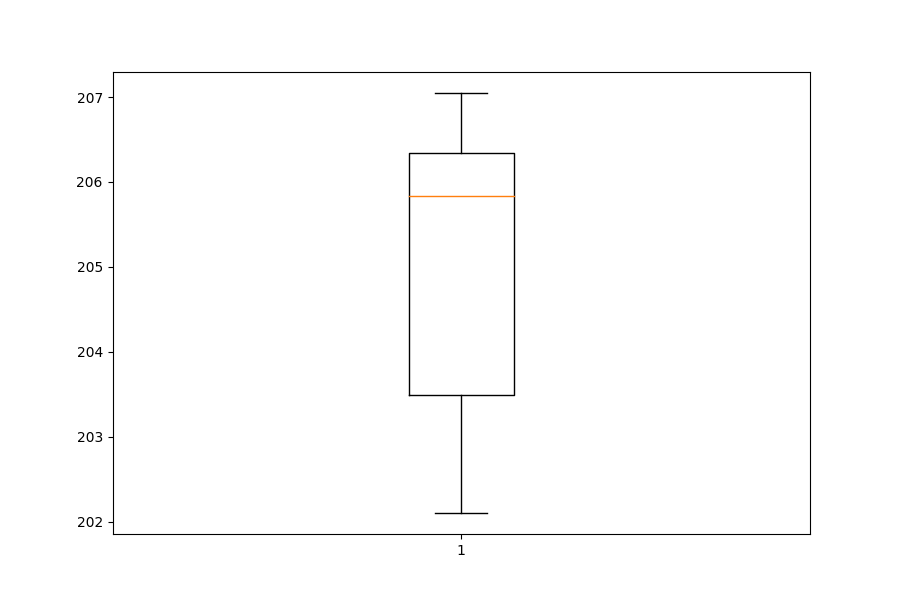
\includegraphics[width=.70\textwidth]{HW10boxplot.png}
	\end{center}
	\caption{Box plot of the given data, Showing no outliers}
   \label{fig:1}
\end{figure}
   
   \subsection*{8}
   \begin{enumerate}[label={\bf \alph*}]
   \item $\bar{X}\pm t_{n-1,\alpha/2}\frac{s}{\sqrt{n}}=196.64 \pm 2.571*\frac{.68}{\sqrt{6}}= 196.64 \pm 0.713$ K
   \item $\bar{X}\pm t_{n-1,\alpha/2}\frac{s}{\sqrt{n}}=196.64 \pm 3.365*\frac{.68}{\sqrt{6}}= 196.64 \pm 0.934$ K
   \item The confidence intervals above would not be valid as what can be seen in figure \ref{fig:2} there is an outlier.
      \begin{figure}[H]
	\begin{center}
		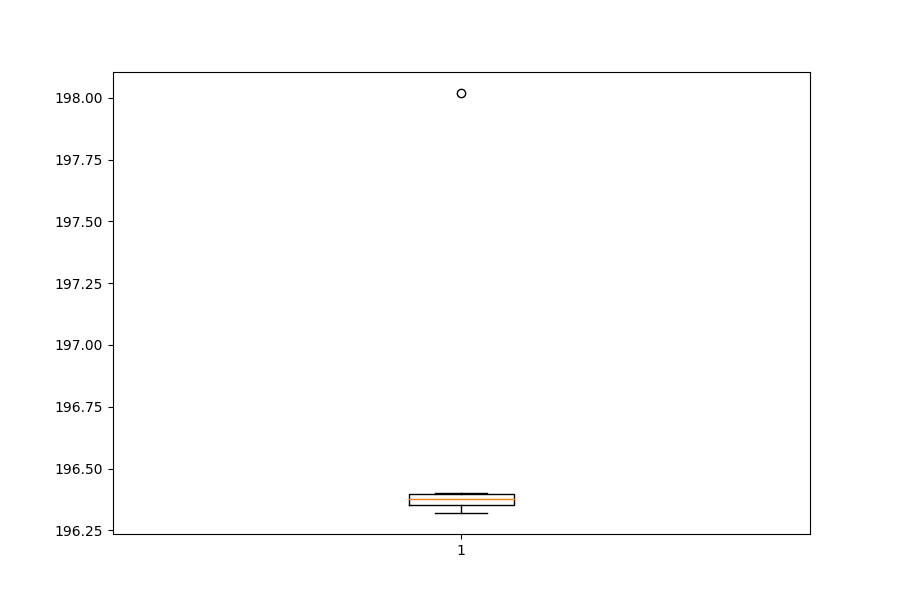
\includegraphics[width=.75\textwidth]{HW10boxplot2.png}
	\end{center}
	\caption{Box plot of the given data, Showing one outlier}
   \label{fig:2}
\end{figure}
   \end{enumerate}
   \subsection*{problem from the lecture}
      For the data given in the lecture there is a CI available the box plot can be seen in figure \ref{fig:3}. The calculation for the 95% CI can be seen below.
   \begin{align*}
      \bar{X}=196.7&68,s= 0.3651\\
      \bar{X}\pm t_{n-1,\alpha/2}\frac{s}{\sqrt{n}}&=196.76 \pm 2.571*\frac{.3651}{\sqrt{6}}\\&=196.76 \pm 0.3832
   \end{align*}
   \begin{figure}[H]
	\begin{center}
		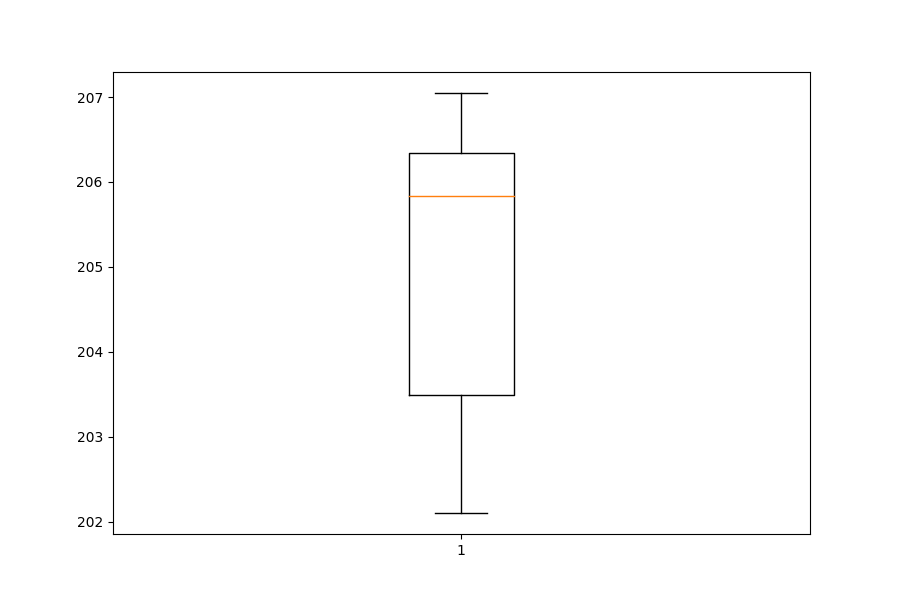
\includegraphics[width=.70\textwidth]{HW10boxplot.png}
	\end{center}
	\caption{Box plot of the given data, Showing no outliers}
   \label{fig:3}
\end{figure}
\end{document}